% !TEX TS-program = XeLaTeX
% use the following command:
% all document files must be coded in UTF-8
\documentclass[portuguese]{textolivre}
% build HTML with: make4ht -e build.lua -c textolivre.cfg -x -u article "fn-in,svg,pic-align"

\journalname{Texto Livre}
\thevolume{17}
%\thenumber{1} % old template
\theyear{2024}
\receiveddate{\DTMdisplaydate{2023}{5}{30}{-1}} % YYYY MM DD
\accepteddate{\DTMdisplaydate{2023}{8}{1}{-1}}
\publisheddate{\DTMdisplaydate{2023}{11}{1}{-1}}
\corrauthor{Lucas Maciel}
\articledoi{10.1590/1983-3652.2024.46380}
%\articleid{NNNN} % if the article ID is not the last 5 numbers of its DOI, provide it using \articleid{} commmand 
% list of available sesscions in the journal: articles, dossier, reports, essays, reviews, interviews, editorial
\articlesessionname{articles}
\runningauthor{Maciel e Gonçalves-Segundo} 
%\editorname{Leonardo Araújo} % old template
\sectioneditorname{Daniervelin Pereira}
\layouteditorname{Thaís Coutinho}

\title{Anões, chads e nazipardos: as estratégias de nomeação e predicação no discurso da direita-alternativa no Brasil}
\othertitle{Anons, chads and mixed-nazis: the naming and predication strategies in the discourse of the alt-right in Brazil}
% if there is a third language title, add here:
%\othertitle{Artikelvorlage zur Einreichung beim Texto Livre Journal}

\author[1]{Lucas Pivetta Maciel~\orcid{0000-0002-6247-037X}\thanks{Email: \href{1.lucaspm@gmail.com}{1.lucaspm@gmail.com}}}
\author[1]{Paulo Roberto Gonçalves-Segundo~\orcid{0000-0002-5592-8098}\thanks{Email: \href{paulosegundo@usp.br}{paulosegundo@usp.br}}}
\affil[1]{Universidade de São Paulo, Faculdade de Filosofia Letras e Ciências Humanas, São Paulo, SP, Brasil.}

\addbibresource{article.bib}
% use biber instead of bibtex
% $ biber article

% used to create dummy text for the template file
\definecolor{dark-gray}{gray}{0.35} % color used to display dummy texts
\usepackage{lipsum}
\SetLipsumParListSurrounders{\colorlet{oldcolor}{.}\color{dark-gray}}{\color{oldcolor}}

% used here only to provide the XeLaTeX and BibTeX logos
\usepackage{hologo}

% if you use multirows in a table, include the multirow package
\usepackage{multirow}

% provides sidewaysfigure environment
\usepackage{rotating}

% CUSTOM EPIGRAPH - BEGIN 
%%% https://tex.stackexchange.com/questions/193178/specific-epigraph-style
\usepackage{epigraph}
\renewcommand\textflush{flushright}
\makeatletter
\newlength\epitextskip
\pretocmd{\@epitext}{\em}{}{}
\apptocmd{\@epitext}{\em}{}{}
\patchcmd{\epigraph}{\@epitext{#1}\\}{\@epitext{#1}\\[\epitextskip]}{}{}
\makeatother
\setlength\epigraphrule{0pt}
\setlength\epitextskip{0.5ex}
\setlength\epigraphwidth{.7\textwidth}
% CUSTOM EPIGRAPH - END

% LANGUAGE - BEGIN
% ARABIC
% for languages that use special fonts, you must provide the typeface that will be used
% \setotherlanguage{arabic}
% \newfontfamily\arabicfont[Script=Arabic]{Amiri}
% \newfontfamily\arabicfontsf[Script=Arabic]{Amiri}
% \newfontfamily\arabicfonttt[Script=Arabic]{Amiri}
%
% in the article, to add arabic text use: \textlang{arabic}{ ... }
%
% RUSSIAN
% for russian text we also need to define fonts with support for Cyrillic script
% \usepackage{fontspec}
% \setotherlanguage{russian}
% \newfontfamily\cyrillicfont{Times New Roman}
% \newfontfamily\cyrillicfontsf{Times New Roman}[Script=Cyrillic]
% \newfontfamily\cyrillicfonttt{Times New Roman}[Script=Cyrillic]
%
% in the text use \begin{russian} ... \end{russian}
% LANGUAGE - END

% EMOJIS - BEGIN
% to use emoticons in your manuscript
% https://stackoverflow.com/questions/190145/how-to-insert-emoticons-in-latex/57076064
% using font Symbola, which has full support
% the font may be downloaded at:
% https://dn-works.com/ufas/
% add to preamble:
% \newfontfamily\Symbola{Symbola}
% in the text use:
% {\Symbola }
% EMOJIS - END

% LABEL REFERENCE TO DESCRIPTIVE LIST - BEGIN
% reference itens in a descriptive list using their labels instead of numbers
% insert the code below in the preambule:
%\makeatletter
%\let\orgdescriptionlabel\descriptionlabel
%\renewcommand*{\descriptionlabel}[1]{%
%  \let\orglabel\label
%  \let\label\@gobble
%  \phantomsection
%  \edef\@currentlabel{#1\unskip}%
%  \let\label\orglabel
%  \orgdescriptionlabel{#1}%
%}
%\makeatother
%
% in your document, use as illustraded here:
%\begin{description}
%  \item[first\label{itm1}] this is only an example;
%  % ...  add more items
%\end{description}
% LABEL REFERENCE TO DESCRIPTIVE LIST - END


% add line numbers for submission
%\usepackage{lineno}
%\linenumbers

\begin{document}
\maketitle

\begin{polyabstract}
\begin{abstract}
O 4chan é um fórum digital conhecido pela forte presença de movimentos de direita-alternativa \cite{nagle2017kill, tuters2018larping}. Neste artigo, a partir da abordagem histórico-discursiva \cite{wodakreisigl2016} dos
estudos críticos do discurso \cite{wodameyer2016}, apresentamos um breve estudo quali-quantitativo sobre
esse fórum em duas partes: em primeiro lugar, discutimos processos de inovação lexical que ocorrem
endemicamente nesse tipo de ambiente digital e, em segundo, apresentamos um panorama que expõe os termos
mais recorrentes na nomeação e predicação de atores sociais representados no discurso nessa plataforma, em
um corpus de 3.675 comentários. A partir desses exemplos, selecionamos casos que representam alguns dos
processos de inovação vernacular mais produtivos, nomeadamente, o desbotamento semântico \cite{peeters2021vernacular}, os blends morfológicos e os significantes flutuantes \cite{tutershagen2020they}. A este último, dedicamos
uma discussão mais detida a partir das instâncias reveladas no corpus deste estudo. Concluímos, a partir desses
dados, que o ambiente é altamente profícuo no uso de jogos de linguagem para representação de atores sociais
tomados como antagonísticos, reproduzindo discursos marcadamente racistas, antissemitas e transfóbicos.

\keywords{Estudos Críticos do Discurso \sep Abordagem Histórico-Discursiva \sep Mídias digitais \sep Alt-right \sep Seleção
lexical}
\end{abstract}

\begin{english}
\begin{abstract}
4chan is a digital forum known for its strong presence of alt-right movements \cite{nagle2017kill, tuters2020esoteric}. In this article, based on the Discourse-historical Approach \cite{wodakreisigl2016} of Critical Discourse
Studies \cite{wodameyer2016}, we present a brief qualitative and quantitative study on this forum in two parts:
first, we discuss processes of lexical innovation that occur endemically in this type of digital environment and,
second, we present an overview that exposes the most recurrent terms in the naming and predication of social
actors represented in the discourse on this platform, in a corpus of 3,675 comments. From these examples, we
selected cases that represent some of the most productive vernacular innovation processes, namely, semantic
fading \cite{peeters2021vernacular}, morphological blends and floating signifiers \cite{tutershagen2020they}. To the
later, we dedicate a more detailed discussion based on the instances revealed in the corpus of this study. We
conclude, based in this data, that the environment is highly fruitful in the use of language games to represent social
actors taken as antagonistic, reproducing markedly racist, antisemitic and transphobic discourses.

\keywords{Critical Discourse Studies \sep Discourse-Historical approach \sep Digital media \sep Alt-right \sep Lexical choice}
\end{abstract}
\end{english}
% if there is another abstract, insert it here using the same scheme
\end{polyabstract}

\section{Introdução}

\emph{Imageboards} são fóruns \emph{online} cuja característica fundamental é a criação de fios de discussão temáticos acompanhados de uma ampla utilização de recursos imagéticos. Os exemplos mais significativos são 8kun, Endchan, Neinchan, 16chan e, com maior destaque, tanto em influência geral quanto em número de usuários, o 4chan \cite{baele2021variations}. Esse último fórum, objeto desta análise, é dividido em boards\footnote{Em português, “painel” ou “página”. Essa subdivisão é comum em fóruns digitais para organização das comunidades em campos de interesse e tópicos de discussão compartilhados.} temáticos, que definem os tipos de discussão realizadas por seus usuários, organizados nas categorias: cultura japonesa, videogames, interesses, criatividade, miscelânea e adulto, conforme são apresentados na página inicial.

Criado em 2003, com base no 2chan, ou Futaba Channel, um fórum \emph{online} japonês, o 4chan, foi inicialmente utilizado como centro de discussão e compartilhamento de conteúdo de \emph{animes} e cultura japonesa. Posteriormente, porém, como aponta \textcite[p. 21, tradução nossa]{nagle2017kill}\footnote{Originalmente: “It became a massively influential and creative forum known for pranks, memes and images that ‘cannot be unseen’. The culture of the site was not only deeply and shockingly misogynist, but also self-deprecating in its own self-mockery of nerdish ‘beta’ male identity. Cultural touchstones included war-based video games and films like Fight Club and The Matrix. There was no registration or login required, so posts were typically all under the username ‘Anonymous’” \cite[p. 21]{nagle2017kill}.}:

\begin{quote}
    tornou-se um fórum massivamente influente e criativo conhecido por pranks, memes e imagens que não podem ser desvistas. A cultura do site não é apenas profunda e chocantemente misógina, mas também autodepreciativa em sua própria autozombaria em relação à identidade macho beta nerd. Marcos culturais da comunidade incluíam videogames baseados em guerras e filmes como Clube da Luta e Matrix. Registro e login não são necessários, então os posts são feitos tipicamente sob o nome de usuário \emph{Anonymous}.
\end{quote}

Devido a esse comportamento considerado anômalo no contexto das mídias digitais \cite{bernstein20114chan}, o 4chan e outros \emph{imageboards}, ainda que em menor extensão, têm se constituído objetos de interesse acadêmico, pelo menos, desde 2010. Além disso,  seus efeitos e impactos têm recebido particular atenção por sua relevância na articulação de movimentos recentes da direita-alternativa [\emph{alt-right}], uma vez que o \emph{imageboard} propicia espaço para discussões racistas, apresenta discurso violento, exerce influência linguística em discursos políticos específicos ou ainda constitui terreno fértil para divulgação e criação de notícias falsas. Segundo \textcite{saklofske2011using}, o 4chan  constitui-se como uma plataforma instável, e sua comunidade está sempre engajada em uma atividade lúdica, em um processo criativo de experimentações e avaliações, imersa em produção de sentidos, ainda que evidentemente repreensíveis.

\textcite{colley2022challenges}, consonantemente, indicam que, no âmbito acadêmico, pelo menos até 2016, a maior parte das pesquisas sobre o 4chan era de caráter antropológico e/ou etnográfico. A partir de então, pesquisas quantitativas, principalmente nas áreas de tecnologia da informação, análise de dados e mídias digitais, como as de \textcite{tutershagen2020they}, \textcite{mittos2020analyzing}, \textcite{baele2021variations} e, anteriormente, \textcite{bernstein20114chan}, passam a ser encontradas com maior frequência. \textcite{colley2022challenges} assinalam, no entanto, a necessidade de pesquisas com foco na análise discursiva e conversacional para revelar e compreender tendências de mobilização interna do fórum, extremamente prolífico, em nossa visão, para a eclosão de discursos com potencial extremista e para a emergência de um vernáculo internamente coeso capaz de mediar e reproduzir a ideologia latente da comunidade que o utiliza \cite{wodakreisigl2016}.

Assim, com base nas ferramentas dispostas pela Abordagem Histórico-Discursiva \cite{wodakreisigl2016} no âmbito geral dos Estudos Críticos do Discurso \cite{wodameyer2016}, propomos uma análise das estratégias de nomeação e predicação dos atores sociais no discurso a fim de compreender de que modo processos linguísticos de seleção e inovação lexical endêmicos à plataforma criam representações próprias do eu e do outro nas interações materializadas nesse espaço. Para isso, devemos pontuar que a plataforma apresenta discussões recorrentes com temáticas étnicas e raciais, com detalhamento acerca de características fenotípicas e genéticas \cite{baele2021variations, mittos2020analyzing}, evidenciando atitudes e posturas notadamente racistas.

Para os fins deste trabalho, portanto, visto que os Estudos Críticos do Discurso se preocupam com o discurso sob a perspectiva da manutenção de estruturas de poder e a resistência em relação a elas, como no caso do discurso racista, adotamos o método proposto por \textcite{wodakreisigl2016} como ferramenta de análise de uma interação entre usuários anônimos que comentaram em 12 fios de discussão em português do 4chan, com enfoque no papel das escolhas lexicais na fundamentação do discurso que motiva essas interações. Como explica \textcite[p. 61, tradução nossa, colchete nosso]{richardson2017british}, “toda análise crítica do discurso busca contextualizar o discurso – analisar e entender o texto em contexto. Previsivelmente, a Abordagem Histórico-Discursiva [AHD] contextualiza o discurso historicamente”, permitindo a análise de textos contemporâneos, compreendidos como, de uma forma ou outra, consequência dos desenvolvimentos da história. 

A AHD propõe cinco níveis de análise para compreender as práticas discursivas de forma crítica – (i) o textual interno, (ii) o intertextual, (iii) o interdiscursivo, (iv) os enquadramentos institucionais e (v) o contexto sociopolítico histórico de forma mais abrangente. Ela apresenta cinco perguntas fundamentais com uma orientação heurística para análise de um conjunto de textos de interesse, a fim de depreender as estratégias empregadas na construção do discurso, isto é, na adoção e no emprego de práticas de representação deliberadas na realização de objetivos linguísticos, sociais e políticos de um grupo social, nomeadamente:

\begin{enumerate}
    \item Como pessoas, objetos, fenômenos/eventos, processos e ações são nomeados e referidos linguisticamente?
    \item Que características e qualidades são atribuídas a esses atores sociais, objetos, fenômenos/eventos e processos?
    \item Que argumentos são mobilizados no discurso em questão?
    \item De que perspectiva essas nomeações, atribuições e argumentos são expressos?
    \item Os respectivos enunciados são articulados manifestamente, isto é, são mitigados ou intensificados?
\end{enumerate}

Neste artigo, parte de uma pesquisa mais ampla voltada ao estudo do discurso (e da argumentação) etnonacionalista na plataforma, detemo-nos tão somente na fase inicial desse trajeto de análise, buscando as respostas para as perguntas 1 e 2, com foco na nomeação e predicação de atores sociais representados no discurso, depreendidos no nível (i) textual interno, partindo das discussões realizadas em língua portuguesa no \emph{board International} do 4chan. Para isso, agregamos ao arcabouço histórico-discursivo as categorias de \textcite{van1996representation}, como graus de especificação, pessoalização, identificação e determinação, a fim de descrever de que modo a seleção lexical consiste em estratégia fundamental de consolidação dessa comunidade discursiva. Dessa forma, buscamos evidenciar as posturas dos participantes do fórum em relação ao seu endo e exogrupo, depreendendo como esses grupos são representados, tendo em vista uma construção guiada por afetos e por estratégias de identificação coletiva, essenciais na diferenciação entre o \emph{eu} e o \emph{outro} no discurso \cite{mouffe2018left}.

Para dar conta de tal investigação, realizamos uma revisão da literatura acadêmica sobre a plataforma entre 2011 e 2022, a fim de definir um conjunto internamente coeso de práticas semióticas estáveis que se constituem no contexto dessa comunidade digital, relacionadas ao tópico central deste estudo. A partir daí, selecionamos nosso \emph{corpus} com um centramento tópico específico, o das discussões de caráter étnico e racial, fundado nas premissas apresentadas a partir da revisão da dinâmica geral da plataforma. Os últimos passos do percurso analítico, finalmente, consistem no objeto central deste artigo, em que realizamos uma análise quali-quantitativa de nossos dados e um estudo detido das categorias de nomeação e predicação mais produtivas desse corpus, definindo seus lugares e funções na representação de atores sociais relevantes nas discussões dessas comunidades. Nesse processo, buscaremos lançar luz às estratégias de constituição de um vernáculo alternativo, debatendo suas implicações na representação, realizada pelos usuários da plataforma, acerca do endo e do exogrupo. 


\section{O 4chan como comunidade discursiva}\label{sec2}

Nesta seção, realizamos um levantamento de dados sobre o 4chan, a fim de caracterizar sua comunidade histórico-discursivamente, indicando brevemente as características políticas geralmente vinculadas ao comportamento de sua comunidade, sua relação com um movimento político comumente entendido como direita-alternativa [\emph{alt-right}] \cite{nagle2017kill} e as características discursivas que o definem como um ambiente que constrói um enquadramento de realidade compartilhado e que emprega práticas semióticas internamente difundidas e estáveis, com ocorrência consistente ao longo das interações nos \emph{boards} analisados. 


\subsection{A direita-alternativa \emph{online}}

A conexão entre o 4chan e a emergência de movimentos políticos extremistas fica evidente com uma análise ampla dos estudos realizados sobre a plataforma até 2023. Nenhum desses estudos, especialmente os publicados depois de 2016, falha em deixar claro não apenas suas motivações, mas também seus resultados, que revelam a produtividade do \emph{imageboard} na geração de engajamento político na contemporaneidade, em especial no âmbito da direita-alternativa.

\textcite{hine2017kek}, por exemplo, evidenciam a grande quantidade de discurso de ódio no 4chan. \textcite{zannettou2018origins}, por seu turno, demonstram o volume de sites de notícias alternativas de direita que são linkados e mencionados na plataforma. \textcite{nagle2017kill} relaciona o 4chan aos conflitos culturais da internet e explica a relevância da plataforma nas eleições americanas de 2016 e a grande presença de personalidades de extrema-direita nas discussões do fórum, argumentando que determinados \emph{boards} de discussão, aliados à cultura de memes e ao discurso linguisticamente alternativo da comunidade, como discutiremos a seguir, deram impulso à maior adesão de jovens ao movimento da direita-alternativa. 

No ano seguinte, \textcite{hagen2018} analisa a volatilidade dos sentimentos políticos presentes na plataforma, exemplificando a ocorrência regular de termos e discussões de caráter antissemita ao longo de anos. Semelhantemente, \textcite{tuters2018larping} discute a criação de símbolos com referências nazistas no 4chan, especialmente a do denominado \emph{Kekistan}, um estado étnico idealizado cujo motivo imagético (\Cref{fig1,fig2}) é baseado na \emph{Reichskriegsflagge} – literalmente, Bandeira de Guerra do Reich –, uma bandeira de guerra nazista. Posteriormente, os autores estudam o uso de representações marcadamente antissemitas e a criação discursiva de um outro nebuloso, evidenciando a fertilidade da plataforma para posturas radicalizadas de seus usuários \cite{tutershagen2020they}.

\begin{figure}[h!]
 \centering
 \begin{minipage}{.45\textwidth}
 \includegraphics[width=\textwidth]{image1.jpg}
 \caption{Kekistan no Brasil.}
 \label{fig1}
 \source{Congresso em Foco (2018).}
 \end{minipage}%
 \qquad
 \begin{minipage}{0.45\textwidth}
 \includegraphics[width=\textwidth]{image2.png}
 \caption{Reichskriegsflagge no Brasil.}
 \label{fig2}
 \source{Congresso em Foco (2018).} 
 \end{minipage}%
\end{figure}


Em 2020, \cite{mittos2020analyzing} analisam um banco de dados sobre discussões de testes genéticos no 4chan e demonstram como esses testes têm se tornado ferramentas que motivam discussões centradas na pureza genética de determinados usuários e suas implicações. Mais especificamente, demonstram como o leite, por exemplo, é associado ao supremacismo branco, devido à (suposta) maior capacidade de genes europeus digerirem lactose. Oportunamente, os autores demonstram como esses mesmos temas geram discussões de diferentes teores em plataformas distintas. No Twitter, por exemplo, comentários sobre testes genéticos estão mais comumente ligados a saúde e tecnologia, enquanto no 4chan as conexões mais comuns são a direita-alternativa e o antissemitismo. \textcite{colley2022challenges}, por sua vez, entendem haver um esforço metapolítico dos usuários da plataforma em deslocar a Janela de Overton, de forma a buscar tornar os temas recorrentemente discutidos na plataforma mais passíveis de discussão no debate público geral. Os autores avaliam haver três acordos fundamentais entre os usuários da comunidade do 4chan: (i) a defesa da liberdade de expressão extrema, (ii) a crença de que a comunidade possui um esclarecimento maior sobre o mundo, (iii) a atitude crítica às hipocrisias do \emph{liberalismo} norte-americano\footnote{Nagle (2017) trata especificamente de \emph{liberalism}, no contexto norte-americano, isto é, uma corrente moderna da doutrina socio-econônima liberal clássica, distinto, portanto, do que se entenderia pelo termo \emph{liberalismo} no Brasil.} \cite{nagle2017kill}.

Adicionalmente, \textcite{elley2021rebirth} argumenta sobre as conexões da comunidade com mitos de superioridade racial e o \emph{Novo Homem} da Itália fascista, relacionando o melhoramento pessoal a ideais de masculinidade tradicionais advindas de uma reinterpretação da cultura clássica. Para o autor, incentivar o bom condicionamento físico, a autossuficiência e o tradicionalismo é essencial para construção do mito fascista de superioridade racial.

Desse modo, notamos uma relação estreita da comunidade discursiva constituída pelos usuários da plataforma com a direita-alternativa. Tal comunidade – vinculando-se a atitudes historicamente inscritas na constituição de um movimento político que, através do antagonismo com setores da própria direita conservadora tradicional e atitudes manifestamente negativas em relação a grupos sociais minoritários, além do explícito vínculo a representações e mobilizações de discursos marcadamente nazistas, antissemitas e racistas de modo amplo – busca constituir uma alternativa política que se constitui não somente pela retomada e reinterpretação de determinadas atitudes socialmente marginais no debate político moderno, mas também pela construção linguístico-discursiva de um ambiente que sustente seus enquadramentos de realidade de modo favorável a seus objetivos políticos, cujo funcionamento discutimos a seguir. 



\subsection{A Rede Vernacular Profunda}

As práticas linguísticas endêmicas ao 4chan pertencem a um ambiente denominado por \textcite{tuters2018larping} como \emph{Rede Vernacular Profunda (Deep Vernacular Web} e emergem de uma comunidade que se compreende como fundadora da cultura digital, como uma comunidade autóctone que se opõe à cultura de informação de massas, cujo escopo abrange usuários de múltiplas plataformas digitais. Essa postura reativa é responsável pela emergência de uma subcultura digital antagonística, que, por meio de múltiplas formas de \emph{gatekeeping}\footnote{O controle da possibilidade de acesso ao discurso em determinadas esferas públicas \cite[p. 25]{wodakreisigl2016}}, dificulta o acesso aos ambientes em que se encontram e afastam-se de outras esferas e comunidades da internet. Uma análise sobre a comunidade discursiva do 4chan, nesse sentido, nos auxilia a compreender alguns desses processos. 

Nesse âmbito, devemos destacar que o interesse pela relação de influência mútua entre as possibilidades e restrições da infraestrutura de um ambiente digital e as práticas discursivas nele emergentes, ou \emph{affordances} \cite{tuters2021meme}, tem ganhado cada vez mais corpo nos estudos das novas mídias digitais. Por isso, julgamos relevante introduzir aqui, valendo-nos do conceito de affordance, alguns pontos sobre as dinâmicas do 4chan que representam os principais exemplos dessa relação meio-prática na plataforma. Para fazer isso, partiremos das características infraestruturais mais ressaltadas pela literatura especializada na plataforma, nomeadamente as implicações da anonimidade e da efemeridade das interações propicias pelo ambiente \cite{bernstein20114chan, saklofske2011using, hine2017kek}), que possibilitam a emergência de um ambiente discursivo que se baseia no antagonismo como fundador de identidade de grupo. 

Em um contexto de anonimidade, os marcadores de capital social se diluem. Sendo assim, a comunidade ancora-se em outros mecanismos de construção de identidade e representação de \emph{status} nas interações \cite{tuters2018larping, tuters2021meme, colley2022challenges}. Outro fator importante que define as práticas discursivas e interacionais no 4chan é a efemeridade dos fios. A maioria dos \emph{boards} tem um limite de 10 páginas, o que faz com que os \emph{posts} mais antigos e com menos engajamento sejam gradualmente retirados das páginas principais, arquivados e, posteriormente, deletados sem possibilidade de recuperação.

Nesse sentido, \textcite{peeters2021vernacular} – valendo-se da noção fundamental de jogos de linguagem de \textcite{witt1958} – argumentam que o \emph{imageboard} em questão é uma plataforma favorável à manutenção de uma comunidade linguística alternativa. Por meio de processos do que ele denomina \emph{Inovação Vernacular Robusta}, referente aos jogos de linguagem recorrentes e generalizados que cunham termos duradouros nas interações da comunidade \cite{peeters2021vernacular}, os usuários sustentam uma comunicação alternativa e, por isso, quase hermética, que obriga que novos usuários passem pelo que pode ser caracterizado como um \emph{letramento subcultural} para entender e interagir de maneira adequada nesses ambientes. 

Entende-se, nesse sentido, que a linguagem passa por uma relação de co-evolução entre os usuários e o contexto em que estão inseridos \cite{peeters2021vernacular}, impedindo um acesso amplo e facilitado a essas comunidades, visto que as discussões são permeadas por processos linguísticos endêmicos de variação e especialização no interior das interações da comunidade.

Os processos de inovação vernacular mais recorrentes podem ser divididos em dois grandes grupos: (i) a criação de neologismos e (ii) a ressignificação de termos. Esses processos, por sua vez, ocorrem em três sentidos diferentes: (a) na criação de terminologia referencial endogrupal e exogrupal, (b) em jogos de palavras e (c) em \emph{performatividade reflexiva}. Cada um desses merece um detalhamento maior, que faremos a seguir.

Saber produzir, interpretar e articular as formas linguísticas internamente consolidadas é parte essencial da aceitação dos membros na comunidade e da solidificação de representações discursivas dos atores sociais relevantes na constituição das comunidades discursivas da plataforma. É comum, por exemplo, que usuários demandem maior conhecimento do vernáculo antes que novos participantes possam fazer postagens originais. Essa demanda por conhecimento das práticas endogrupais se evidencia também pela ênfase que as diretrizes de alguns \emph{boards} estabelecem sobre o conteúdo original, solicitando que os usuários estejam atentos aos fios já existentes antes de criar novos, reforçando a necessidade de um letramento particular e de uma familiarização com as práticas discursivas desse espaço digital para participar efetivamente nas discussões do fórum. 

Como no 4chan as comunidades não têm propriedade definida e há intensa pluralidade temática, a sua identidade acaba se definindo por outros fatores. Dentre eles, destacamos as práticas antagonísticas voltadas à criação discursiva de um eu em oposição a um \emph{outro} \cite{tutershagen2020they, elley2021rebirth}, evidenciada pela especialização das estratégias de nomeação e predicação dos objetos do discurso.

Essa construção pode ser observada, por exemplo, na emergência do vernáculo inovador e alternativo, que já mencionamos. Na plataforma, o fato de serem mais frequentes expressões nominais que fazem referência ao \emph{endogrupo} em comparação ao \emph{exogrupo} \cite{peeters2021vernacular} parece indicar uma movimentação de diferenciação cultural e construção de uma identidade compartilhada. Esses termos comunitários serão comumente autodepreciativos e, não raro, constituirão ressignificações de termos depreciativos. O afixo -\emph{fag} (bicha/viado), por exemplo, é frequentemente recrutado para derivar formas de nomeação dos membros do endogrupo. Um exemplo são os usuários novos, denominados \emph{newfags}, e os antigos, \emph{oldfags}. 

Já no caso da nomeação \emph{exogrupal}, observamos uma ampla apropriação de termos que refletem o antagonismo da comunidade em relação a determinados grupos étnicos. Parte significativa desses termos passa por um processo de \emph{desbotamento semântico} \cite{sweetser1988grammaticalization}, tornando-os distintos de seu significado original e funcionando no contexto das práticas discursivas dessa subcultura. 

Os jogos de palavras, como definidos por \textcite{peeters2021vernacular}, por sua vez, são parte fundamental da manutenção do \emph{gatekeeping} dessa comunidade, funcionando não apenas como uma forma de tornar o discurso ambíguo e vago, mas como forma de dificultar o acesso à cultura dos \emph{chans}. O \emph{corpus} que apresentaremos a seguir indica que várias palavras são propositalmente usadas com variações ortográficas que induzem reinterpretações dos significados típicos a elas associados, não raro em termos de ironia. Alguns exemplos desses casos seriam \emph{raep (rape), moar (more)} e \emph{rekt (wrecked)}\footnote{Em português, “estupro”, “mais” e “destruído”, respectivamente.}. Esse tipo de jogo de palavras dificulta a avaliação das intenções reais de seus usuários e possibilita que os usuários do fórum rebatam análises críticas sobre os padrões de linguagem por eles empregados sob o pretexto de se tratar de um uso humorístico e despretensioso. 

Por último, \emph{reflexividade performativa} refere-se à terminologia empregada para representar e avaliar os aspectos infraestruturais da plataforma e os usos que os participantes fazem das possibilidades técnicas \cite[p. 10]{peeters2021vernacular}. O nome \emph{tripbicha}, por exemplo, que mostraremos posteriormente, indica a postura negativa da comunidade em relação aos usuários que, em vez de permanecer absolutamente anônimos (sob o usuário padrão anonymous), utilizam os identificadores \emph{tripcodes}, sequências numéricas aleatórias que identificam um usuário nos fios de discussão.

Além disso, tendo em vista a descentralidade dos perfis dos membros dessa subcultura, \textcite{tutershagen2020they} propõem que \emph{significantes flutuantes} são parte importante do estabelecimento de uma identidade para a comunidade, isto é, “aqueles significantes que absorvem em vez de emitir significado e são suscetíveis a interpretações múltiplas ou até contrárias” \cite[p. 2230]{tutershagen2020they}. Os autores pontuam, sobretudo, que o outro estabelecido discursivamente terá um caráter nebuloso, isto é, vago e aberto à interpretação dos usuários. Nesse sentido, percebemos como a abertura apresentada por um \emph{significante flutuante} é o que permite que uma comunidade descentralizada com diversos sentimentos políticos encontre um objeto comum em que investe coletivamente na criação de uma rede de conexões e negociações de pertencimento \emph{endogrupal}, especialmente em contexto de anonimidade, como discutimos adiante.

Isso posto, trataremos, na próxima seção, dos aspectos teórico-metodológicos que guiam nossa análise quali-quantitativa dos dados. Guia a nossa discussão a seguinte pergunta: de que modo os processos gerais de inovação e uso de práticas da \emph{Rede Vernacular Profunda} ocorrem nas estratégias de nomeação e predicação de uma subcomunidade com características linguísticas, sociais e culturais próprias? 



\section{Nomeação e predicação: uma visão geral}

O \emph{corpus} deste estudo é composto por 12 fios extraídos do \emph{board} de discussão \emph{International}, onde podemos encontrar discussões em português, conduzidas, a princípio, por usuários brasileiros da plataforma. Esses 12 fios, que abrangem um total de 3.675 comentários, abarcam discussões com algum tipo de centração tópica de caráter étnico e racial. A partir desse material, abordamos a seleção lexical observada nas interações com uma orientação de crítica sócio-diagnóstica \cite[p. 25]{wodakreisigl2016}, na medida em que tratamos de depreender o caráter discursivo latente através da análise linguística focada. 

Trataremos, assim, o uso do léxico como uma estratégia deliberada de manipulação e manutenção do discurso, seja de forma latente ou manifesta, isto é, se os posicionamentos são explicitamente evidenciados nos enunciados ou se são depreendidos através das formas de representação empregadas. 

A abordagem Histórico-Discursiva propõe um método de triangulação em quatro níveis: o primeiro abrange o co-texto e o co-discurso interno imediato; o segundo, a intertextualidade e as relações interdiscursivas entre enunciados, textos, gêneros e discursos; o terceiro, as variáveis extralinguísticas e os enquadramentos institucionais de um “contexto situacional”; e o quarto, o contexto histórico e sociopolítico mais amplo, em que as práticas discursivas estão vinculadas e relacionadas \cite[p. 93]{wodakreisigl2016}.

Neste artigo em específico, realizamos uma análise partindo de elementos centrados em interações conversacionais localizadas topicamente delimitadas em direção a uma análise mais geral subsequente. Assim, detemo-nos, especialmente, no primeiro nível, a fim de evidenciar as diferentes posições que podem ser identificadas comparativamente quanto ao uso do léxico de um comentário em oposição aos outros e quanto à seleção e modificação de itens lexicais que constituem os jogos de linguagem da \emph{Rede Vernacular Profunda}, construindo, ao longo do processo, relações com o segundo nível, particularmente no que se refere à relação entre a nomeação e a predicação de atores sociais representados e o discurso etnonacionalista da direita alternativa que integra o fórum.

Fazemos a raspagem dos dados por meio de um método ascedente [\emph{bottom-up}], extraindo as informações da plataforma e as organizando de modo estruturado, partindo de interações topicamente centradas que estabelecemos como pontos de partida para uma análise global. Inicialmente, fizemos uma coleta manual de nomes em dois grupos principais de nosso interesse:

\begin{enumerate}
    \item Um grupo relativo ao recorte tópico etnonacionalista, com nomes:
\begin{enumerate}[label=\alph*)]
    \item Étnicos;
    \item Gentílicos;
    \item Fenotípicos\footnote{O grupo “fenotípico” difere do grupo “étnico” na medida em que contempla especificamente nomes que se referem tão somente a características físicas dos atores nomeados.}, que se referem ao outro na interação.
\end{enumerate}
\item Outras formas de nomeação produtivas nas interações, especialmente formas impolidas, subdivididas em três grupos que se mostraram relevantes: 
\begin{enumerate}[label=\alph*)]
    \item Impolidez genérica
    \item Sexo e sexualidade e;
    \item Inovações endêmicas ao 4chan
\end{enumerate}
\end{enumerate}

A primeira parte da coleta foi realizada apenas nas cadeias conversacionais que apresentavam discussões com centramento tópico étnico-racial, muito frequente no \emph{board} temático em questão. Desse recorte, coletamos os nomes apresentados na \Cref{tab1}.


\begin{table}[h!]
\caption{Ocorrências individuais categorizadas}
\label{tab1}
\begin{tabular}{llllll}
\rowcolor[HTML]{FFFFFF} 
\toprule
Gentílico & Endêmico & Étnico & Impolido & Fenotípico & Sexual \\
\midrule
\cellcolor[HTML]{EFEFEF}europeu (5) & white pardo & \cellcolor[HTML]{EFEFEF}índio (6) & imbecil &\cellcolor[HTML]{EFEFEF} preto (6) & \cellcolor[HTML]{FFFFFF}viado \\
tuga & \cellcolor[HTML]{EFEFEF}anão (6) & tamoio & \cellcolor[HTML]{EFEFEF}abominação (2) & escurinho & pedófilo \\
norte-africano (2) & esquizo (2) & \cellcolor[HTML]{FFFFFF}mulatinho & \cellcolor[HTML]{FFFFFF}criaturas & branco (7) & \cellcolor[HTML]{FFFFFF}virgem \\
americano (2) & \cellcolor[HTML]{FFFFFF}bostilhas & \cellcolor[HTML]{FFFFFF}trirracial & aberração (2) & negro (3) & \cellcolor[HTML]{FFFFFF}travequinha \\
\cellcolor[HTML]{FFFFFF}libanês & chad (3) & indígena (2) & chimpanzé (2) & pardo (4) & cuck (2) \\
gaúcho & mutt & \cellcolor[HTML]{EFEFEF}miscigenado (2) & macaquinha & pardito & \cellcolor[HTML]{EFEFEF}tranny (2) \\
\cellcolor[HTML]{EFEFEF}ibérico (2) & mystery meat & \cellcolor[HTML]{EFEFEF}caboclo (2) & chimpa & amarelo &  \\
\cellcolor[HTML]{EFEFEF}germânico (3) & vermelhopilado & berbere & símio & marronzito &  \\
japonês (2) & larp (2) & \cellcolor[HTML]{FFFFFF}árabe & macaco (6) & \cellcolor[HTML]{FFFFFF}negão &   \\
pernambucanos & normie & \cellcolor[HTML]{EFEFEF}mestiço (3) & sub-humano & branquelo &  \\
carioca & nazipardo & birracial & verme &  &  \\
\cellcolor[HTML]{EFEFEF}brasileiro (4) & mogar & mulato & \cellcolor[HTML]{EFEFEF}retardado (2) &  &  \\
afro & tripbicha & mestição & paspalho &  &  \\
pomerano & \cellcolor[HTML]{EFEFEF}bostileiro (2) & afro-brasileira & bonobos &  &  \\
bávaro & chimpanzileiro & \cellcolor[HTML]{EFEFEF}ariano (3) &  &  &  \\
\cellcolor[HTML]{EFEFEF}nordestino (2) & \cellcolor[HTML]{EFEFEF}senpaiília (5) & muçulmano &  &  &  \\
\cellcolor[HTML]{EFEFEF}asiático (2) & inbred & \cellcolor[HTML]{EFEFEF}judeus (3) &  &  &  \\ 
\cellcolor[HTML]{EFEFEF}africano (3) & tranóide & eslavo &  &  &  \\
iraniano & redpill & han &  &  &  \\
etíopes & ;\textasciicircum{}) & \cellcolor[HTML]{EFEFEF}caucasóide (2) &  &  &  \\
paulista & \cellcolor[HTML]{EFEFEF}anon (2) & aborígene &  &  &  \\
sulista & normalfag & Mischling &  &  &  \\
nórdico & snownigger &  &  &  &  \\
japinha & incel &  &  &  &  \\
indiano & v\textasciicircum{}\} &  &  &  &  \\
grego & /Bra/sileiros &  &  &  &  \\
romano & based &  &  &  &  \\
meds &  &  &  &  &  \\
subsaarianos &  &  &  &  &  \\
\bottomrule
\end{tabular}
\source{Elaboração Própria.}
\end{table}

Em primeiro lugar, notamos que se destacam, dentre as categorias que delimitamos, os nomes gentílicos, as inovações endêmicas à plataforma e os nomes étnicos. Os gentílicos foram os mais recorrentes na nomeação de atores do discurso vinculados ao exogrupo. Dada a alta especialização dos nomes \cite{van1996representation}, há uma grande variedade, constituindo-se no grupo de nomeação mais diverso. A categoria das inovações endêmicas ao 4chan também apresenta grande diversidade, porém, como veremos a seguir, elas ocorrem generalizadamente, constituindo-se em estratégias produtivas de nomeação tanto endo quanto exogrupal. Por fim, o grupo de nomes étnicos é extremamente produtivo para referir-se a grupos pouco determinados. 

Em termos das categorias menos produtivas, observamos, no âmbito dos nomes impolidos, um grande volume de nomes de primatas – \emph{chimpanzé, símio, babuíno, bonobo} – usados especialmente na nomeação do endogrupo dos próprios usuários dos fios de discussão em questão como estratégia de autodepreciação. Os nomes fenotípicos, por sua vez, ainda que apresentem menor variedade, são os que apresentam maior número de ocorrência individuais, processo de que trataremos a seguir, e, naturalmente, apresentando alta indeterminação e baixa especificação, descrevendo atores sociais em categorias altamente genéricas, como branco e negro. O último grupo, certamente, é o que constitui a estratégia de nomeação mais anômala nessas discussões, visto que, ainda que nenhum dos textos analisados tenha centramento tópico relativo a sexo ou sexualidade, nomes como \emph{cuck}\footnote{Corno.} e \emph{tranny}\footnote{Derrogatório comum para transexual.} são enunciados com frequência na nomeação antagonística endogrupal entre os usuários.

A partir dessa lista, selecionamos todos os nomes que ocorrem em mais de uma interação, como indicado pelos números e pelas células cinzas na \Cref{tab1}. Fizemos uma busca de cada um desses nomes em todos os \textbf{3.675} comentários de cada um dos \textbf{12} fios de onde foram extraídas as discussões focadas e anotamos seu número de ocorrências. Podemos visualizar os resultados na \Cref{fig3}: 

\begin{figure}[h!]
\centering
\begin{minipage}{.8\textwidth}
 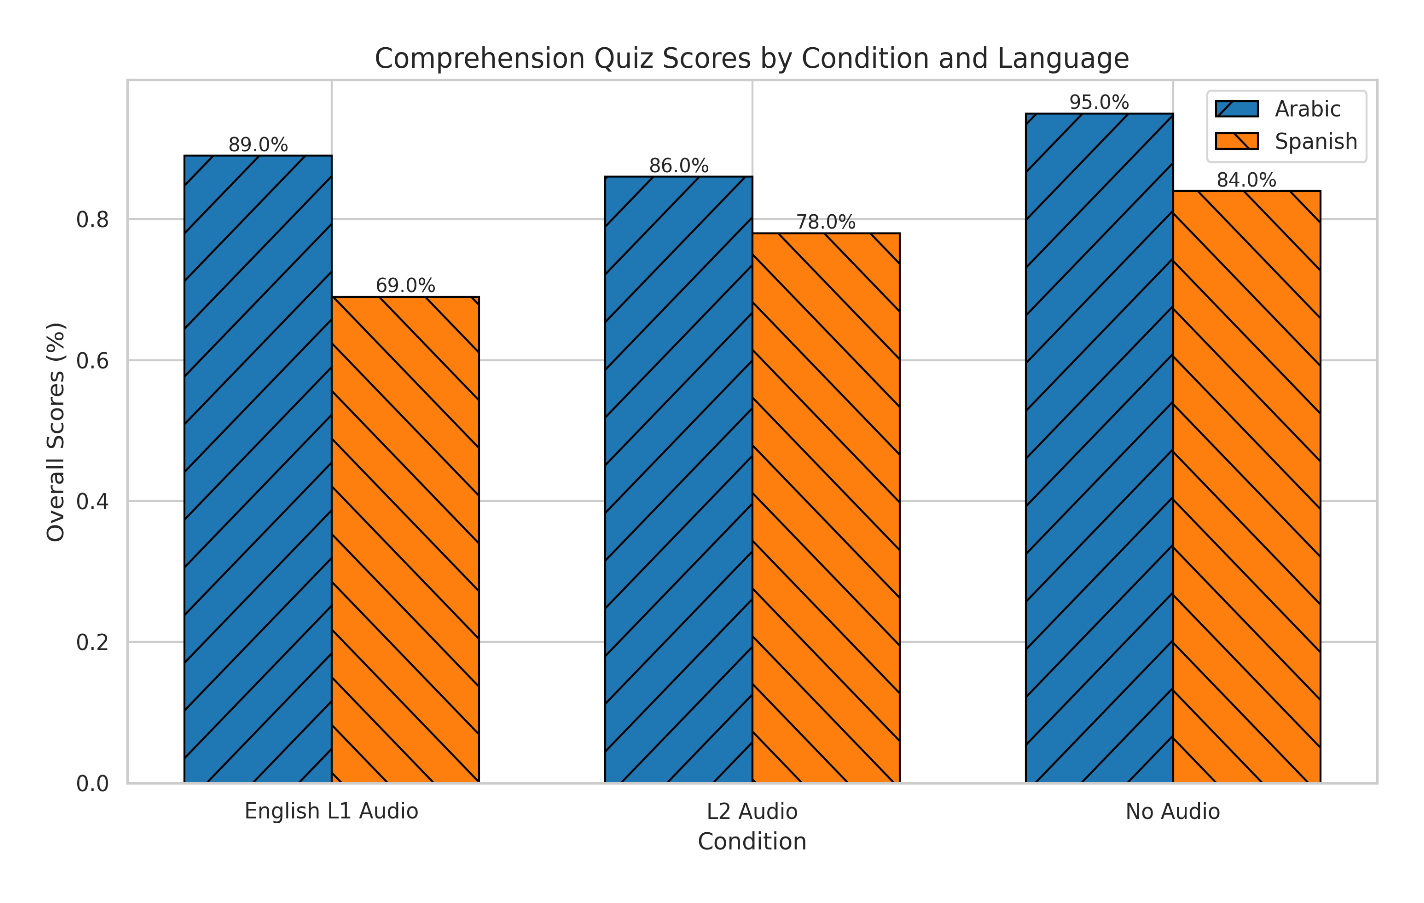
\includegraphics[width=\textwidth]{image3.png}
 \caption[Ocorrência dos nomes selecionados]{Ocorrências individuais dos nomes selecionados\footnotemark.}
 \label{fig3}
 \source{Elaboração própria.}
\end{minipage}
\end{figure}
\footnotetext{O gráfico apresenta apenas os nomes com mais de dez ocorrências.}

Selecionamos, então, todos os nomes com mais de dez ocorrências individuais, a fim de analisar apenas os termos mais recorrentes no \emph{corpus}, e anotamos suas variações e predicações com clara atitude negativa ou positiva e aquelas relativas ao campo semântico étnico-racial (\Cref{tab2}).

\begin{longtable}{llll}
\caption{Predicação de nomes recorrentes e variantes}
\label{tab2}
\\
\toprule
Nome & Predicação & Variantes & \\
\midrule
\multirow{5}{*}{Branco} & ariano da iuropa & Ø & \\ 
& amigos… \\ 
& puros\\ 
& do brasil\\ 
& estudante de engenharia na usp \\
\midrule
\multirow{11}{*}{Judeu} & não brinca em serviço & O judeu {[}3{]} & \\
& coisa de … & Jude {[}1{]} & \\ 
& étnicos & j*deu {[}1{]} & \\ 
& que habitam países germânicos\\ 
& picas\\ 
& com fenótipo 100\% judeus\\ 
& tunisiano\\ 
& bosta\\ 
& mestrerraça dono de bancos e vencedor de nobel\\ 
& do oriente médio\\ 
& \multicolumn{1}{p{7cm}}{{[}são literalmente quem estão tentando fazer um revisionismo histórico e tentando transformar nazismo em direita{]}} \\ 
& são a verdadeira raça superior (irônico) \\
\midrule
Brasileiro & verdadeiro & Ø & \\
 & médio \\
 & mestço \\
 & de alt-right é muito patético \\ 
 & cultura pardoleira … 
 & de elite … \\ 
 & vira latas \\
 \midrule
Europeu & fenótipo… & Sul-europeu {[}1{]} \\
 & traços…\\ 
 & genes… \\
 \midrule
Pardo & anon & Pardocel {[}1{]} & Pardola {[}1{]} \\
 & de 87 de QI & White pardo {[}1{]} \\ 
 & gay pedófilo e schizo & Pardoleira {[}2{]} \\ 
 & nordestino & Pardelícia {[}1{]} \\ 
 & baixo QI & Pardozil {[}1{]} \\ 
 & imprudente & Pardito {[}1{]} \\
 \midrule
Germânico & “bárbaro” & Ø \\  
 & superior \\
 \midrule
Nordestino & de cu ardido & Ø \\ 
 & fudido … é tudo feio pra krl \\
 & e macaco\\ 
 & de pinto pequeno\\ 
 & peão …\\ 
 & de 80 de qi \\
 \midrule
Preto & corno &  Ø \\ 
 & que reclama de morar em favela\\ 
 & pinto pequeno \\ 
 & refugiado\\ 
 & americano \\
 \midrule
Negro & baixo QI  \\
\midrule
Miscigenado & abominação… & Ø \\ 
 & povo…da sua região\\ 
 & imundo\\
 & literalmente\\ 
 & macaco \\
 \midrule
Mestiço & abominável & mestição {[}1{]}\\ 
 & nojento \\ 
 & inferior \\
 \midrule
Africano & lutando pelos nazistas & afro {[}1{]} \\
 & subsaarianos & afro-brasileiro {[}2{]} \\ 
 & é burro \\
 \midrule
Anão & pardo & anon {[}≡{]} \\ 
 & que parece guria \\ 
 & branco\\ 
 & baseado\\ 
 & médio \\
 \midrule
Macaco & chupador de rola & macaquinha {[}1{]} \\
 & treinado para imitar humanos \\ 
 & 87\% europeus\\ 
 & genes de…\\ 
 & de imitação\\ 
 & supremo\\ 
 & pipizinho pequeno\\ 
 & trombadinha\\ 
 & com qi de babuíno pseudo-intelectual\\ 
 & que saiu do nível retardado \\
 \midrule
Humano & sub & sub humano {[}4{]} & \\
\midrule
Corno & postador de pornô & cuck {[}1{]}\\
 & sem vergonha & cuckold {[}1{]}\\ 
 & preto & cucka v. {[}1{]}\\
 & negão & cuckos {[}1{]}\\
 & \multicolumn{1}{p{7cm}}{que paga pela vigésima primeira mansão dos Rothschilds todo mês} & cuckal {[}1{]}
 &DNA de… \\
 \midrule
Transsexual & Ø & traveco {[}6{]} \\
 & & travequinha {[}3{]}\\ 
 & & travequeiro {[}1{]}\\ 
 & & travecoposting {[}1{]}\\ 
 & & travesti {[}1{]}\\ 
 & & trannie {[}3{]}\\ 
 & & tranóide {[}1{]}  \\
 \midrule
Chad & postam no bra & chadessexuais {[}1{]} \\ 
 & …Gomes\\ 
 & …Emílio Medici\\ 
 & gênio\\ 
 & \multicolumn{1}{p{7cm}}{cara ruivo…extremamente inteligente e baseado} \\ 
 \midrule
Senpaiília & real & Ø \\ 
 & safra \\ 
 & de judeus tunisianos \\
 \midrule
Bostileiro & vira-latas & Ø \\ 
 & eugenistas\\ 
 & mediano\\ 
 & odeia trabalhar \\
 \midrule
Retardado & mulheres… & Ø \\ 
 & do PSOL\\ 
 & de 80 de QI \\
\bottomrule
\source{Elaboração própria.}
\end{longtable}


Dispor de uma lista de formas produtivas de nomeação e predicação, topicamente centrada, consiste em um ponto de partida relevante para uma análise orientada da língua para o discurso [\emph{bottom-up}]. Começando com um método centrado nas relações imediatas do léxico no texto, e a partir de um inventário geral, constituído pela \Cref{tab1} e \Cref{tab2}, pudemos definir características globais das estratégias de nomeação e, posteriormente, dispondo dessas listas que incluem as predicações, pudemos utilizar uma abordagem mais ampla, a fim de descrever de modo mais detido quais motivações discursivas permeavam essas escolhas e inovações lexicais e seu papel no discurso da comunidade. Aqui, claro, restringimo-nos a uma visão geral apenas da dimensão de representação linguística dos atores sociais nas discussões.

Parte significativa dos atores representados nessas interações são predicados e nomeados em termos de identificação física, especialmente de teor étnico racial, e como aponta \textcite[p. 58, tradução nossa]{van1996representation}, “a fronteira entre identificação física e classificação está longe de ser clara, como é óbvio pelo uso de cor de pele ou conotações que apoiam-se a tais representações” na nomeação de grupos sociais. É interessante notar, ainda, como a categoria de nomes referentes à sexualidade sociais é produtiva, em termos predicativos, para agregar significados de ridicularização e depreciação a atores representados, no núcleo nominal, por outras categorias, como em: \emph{pardo gay pedófilo, nordestino pinto pequeno, preto corno} e \emph{macaco chupador de rola}. Ressaltamos ainda a grande variação de nomes referentes à transexualidade, como: \emph{tranóide, tranny} e \emph{traveco}. 

Finalmente, o alto número de ocorrências de anão e anon, termo usado para nomear os próprios usuários da plataforma, indicam como os processos de inovação lexical advindos das práticas endogrupais são produtivos, estáveis e difundidos pela comunidade de uso, que se refere a si mesma a partir de nomes especializados, que a distingue como um nós internamente definido.

A seguir, apresentamos uma seção acerca de casos representativos das estratégias endêmicas do 4chan mais estáveis e produtivas na plataforma, e discutimos, ainda que brevemente, possíveis interpretações desses usos em face da literatura relevante sobre a plataforma que apresentamos na seção \ref{sec2}. Começamos por um olhar geral acerca do funcionamento da \emph{Rede Vernacular Profunda} e, posteriormente, tratamos de três fenômenos de destaque na literatura que se fazem igualmente relevantes na comunidade brasileira.


\section{Jogos de linguagem}

Tendo em mente a discussão realizada anteriormente, apresentamos um fluxograma (\Cref{fig4}) que busca sintetizar as práticas linguísticas mais comuns da comunidade da plataforma.

\begin{figure}[h!]
\centering
\begin{minipage}{.8\textwidth}
 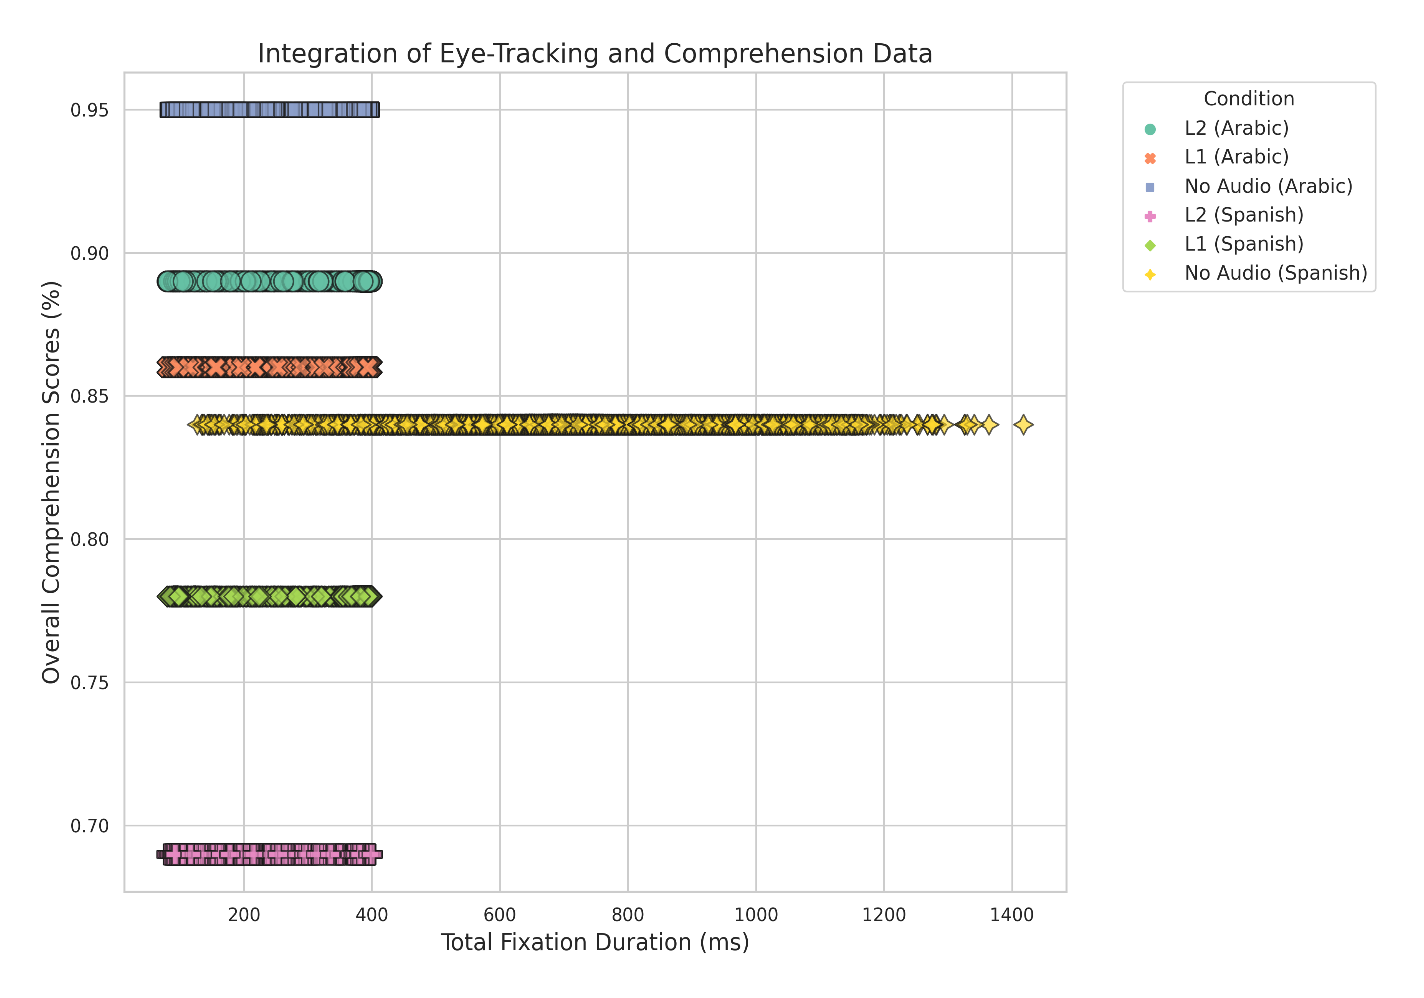
\includegraphics[width=\textwidth]{image4.png}
 \caption{Fluxograma básico de jogos de linguagem no 4chan}
 \label{fig4}
 \source{Elaboração própria, baseado em Peeters et al (2021) e Tuters e Hagen (2020).}
\end{minipage}
\end{figure}

Com base na \Cref{fig4}, buscamos demonstrar a circularidade dos processos de inovação vernacular, evidenciando o caráter de retroalimentação que ocorre nas práticas comunicativas possibilitadas pelos \emph{affordances} da plataforma. Ainda que sinteticamente, podemos observar a relação multidirecional entre os processos linguísticos que ocorrem na plataforma, o que evidencia uma dinâmica interna bem definida, com claros padrões observáveis, cujo funcionamento estabelece uma comunidade de uso muito bem delimitada, fortalecida pelas múltiplas iterações desses mesmos processos. 

Notamos, nesse sentido, que a comunidade de uso da \emph{Rede Vernacular Profunda} alimenta uma necessidade constante de letramento e reutilização desse mesmo léxico inovador. Com isso, tende-se a criar um vernáculo constantemente mais especializado, o que promove \emph{gatekeeping}, ou seja, o controle do acesso à participação efetiva nas práticas discursivas da comunidade.

A partir dessa perspectiva global, informada pela nossa análise \emph{bottom-up} das interações, podemos selecionar alguns casos específicos que representem instâncias produtivas dessas estratégias de nomeação e predicação. Assim, a seguir, apresentamos três processos mais especializados que ocorrem neste \emph{corpus}, nomeadamente: 

\begin{enumerate}
    \item a criação de representações nebulosas do outro; 
    \item as ocorrências de \emph{blends} morfológicos e seu papel na manutenção do discurso; e 
    \item a grande proliferação de nomes marcadamente impolidos na nomeação – especialmente – endogrupal. 
\end{enumerate}


\subsection{O \emph{outro nebuloso}}

As 50 ocorrências do nome judeu é um fenômeno esperado, tendo em vista a literatura existente que aponta o grande volume de sentimento antissemita na plataforma \cite{nagle2017kill, tuters2018larping}. As estratégias de predicação e os tópicos gerais das discussões em que esses nomes são enunciados indicam os pontos de dissenso mais latentes que envolvem os nomes relativos a (i) tópicos étnico-raciais – étnicos, que habitam países germânicos, com fenótipo \emph{100\% judeu, tunisiano} – e (ii) alguns estereótipos referentes a caricaturas de comunidades judaicas que circulam na plataforma – \emph{não brinca em serviço, coisa de…, picas, mestrerraça\footnote{Master race: Raça superior.} dono de banco e vencedor de nobel}. Tendo em vista esse sentimento geral, destacamos três estratégias específicas de nomeação desses atores sociais que são produtivas para compreender as dinâmicas de inovação vernacular exogrupal no 4chan, aquelas que nomeiam o \emph{outro}.

Uma estratégia reiterada, objeto central do estudo conduzido por \cite{tutershagen2020they}, é o uso dos três parênteses ao redor de um nome. Ainda que tenha surgido a partir de uma atitude explicitamente antissemita, esse marcador é usado principalmente com o objetivo de antagonizar de forma ambígua um inimigo comum de que se deve suspeitar – o outro nebuloso. A ocorrência frequente da terceira pessoa do plural – \emph{(((they)))}\footnote{3ª pl. nom. e 3ª pl. ac., respectivamente.} e \emph{(((them)))} – indica como os usuários fazem referência a um outro não definido relativo ao falante, possibilitando que os interlocutores projetem seus sentimentos políticos nessa abertura proporcionada pelo significante flutuante, o que viabiliza a emergência de uma comunidade unida por um antagonista (aparentemente) comum. Em nosso \emph{corpus}, encontramos três ocorrências dessa estratégia:

\begin{enumerate}[label=\alph*)]
    \item Nem sou ele mas ai tá dito que tem uns 26 conceitos de espécie. Nem \textbf{(((consenso)))} tem. Alias, etnia é algo reconhecido. (negrito nosso)
    \item ciência, "ciência" ou \textbf{(((ciência)))}? (negrito nosso)
    \item \textbf{(((Eles)))} ou apenas "Eles"? (negrito nosso)
\end{enumerate}

Os casos \textbf{b} e \textbf{c} representam um uso claro da construção do outro nebuloso. Nas duas ocorrências, os nomes entre parênteses são colocados em direta oposição aos nomes sem as marcações, indicando que existe, primeiro, uma \emph{ciência} e um eles conhecido, pacífico, com significado definido e dois outros referentes opostos, desconhecidos, ocultos e \emph{nebulosos}. 

Conforme apontado por \textcite{tutershagen2020they}, o conteúdo explicitamente antissemita que origina o meme é diluído e quase totalmente apagado; o conteúdo que resta é o caráter negativo com o qual os enunciadores referem-se aos nomes marcados. No caso \textbf{b}, o argumentador refere-se aos dados mobilizados por seu antagonista como uma possível \emph{(((ciência)))}, que avalia negativamente sem explicitar suas razões. O caso c funciona similarmente, visto que o produtor atribui os problemas apontados por seu antagonista são decorrentes de um \emph{(((eles)))} desconhecido. Essa indefinição sobre o referente possibilita uma ampla possibilidade de significação por parte dos participantes do fórum, além de possibilitar que a voz autoral não se comprometa diretamente com uma posição explícita.

Outra estratégia relevante na construção desse \emph{outro nebuloso} constitui-se em processos de \emph{abstração memética}. Para entender esse processo, primeiro, observemos a \Cref{fig5}.

\begin{figure}[h!]
\centering
\begin{minipage}{.8\textwidth}
 \includegraphics[width=\textwidth]{image5.png}
 \caption{Variação do meme \emph{Happy Merchant}}
 \label{fig5}
 \source{ A e B de \textcite{tutershagen2020they}; C e D\footnote{Imagens rotacionadas 90º para a direita.} de 4chan.org/int (Indisponível).}
\end{minipage}
\end{figure}

A versão \textbf{(B)}, chamada de minimalista por Tuters e Hagen (2020), constitui uma ocorrência de \emph{abstração memética}. A mudança da imagem original \textbf{(A)} para uma versão extremamente reduzida faz com que os elementos da gramática memética sejam isolados até um ponto em que a figura se torna completamente incompreensível para grupos não habituados com os jogos de linguagem e referências circulantes da plataforma. 

Semelhantemente, as Figuras \textbf{(C)} e \textbf{(D)} representam outros dois casos de abstração. Em nosso \emph{corpus}, encontramos apenas uma ocorrência de cada e a observação da dinâmica geral da comunidade na plataforma também não indica que alguma das duas formas seja produtiva. De qualquer maneira, são casos que indicam a relevância da proposta dos autores quanto a esse fenômeno no 4chan. A forma \textbf{(C)} ocorre no seguinte complexo oracional:

\begin{quote}
    Então explique por que a maioria dos judeus picas \textbf{v\textasciicircum{}} vem de países germânicos e pouqíssimos vêm de norte da áfrica ou oriente médio que SEMPRE tiveram grandes comunidades judaicas? (negrito nosso)
\end{quote}

Nesse caso, o referente está explicitamente indicado pelo sintagma nominal precedente –– a maioria dos \emph{judeus picas}. Por isso, nesse caso específico, não parece haver o uso da construção do \emph{outro nebuloso}. A forma \textbf{(D)}, no entanto, parece se encaixar no funcionamento proposto pelos autores. Essa forma ocorre em um complexo oracional com uma imagem anexa \Cref{fig6}:

\begin{quote}
    Se vc pensa, logo existe, né \textbf{;\textasciicircum{})} ? (negrito nosso)
\end{quote}

\begin{figure}[h!]
\centering
\begin{minipage}{.6\textwidth}
 \includegraphics[width=\textwidth]{image6.png}
 \caption{Imagem anexa}
 \label{fig6}
 \source{4chan.org/int (Indisponível).}
\end{minipage}
\end{figure}

No comentário acima, notamos a mobilização de um topos argumentativo comum do discurso antissemita. \emph{Pensar}, como ironicamente mobilizado pelo enunciador, é colocado em contradição com uma suposta manipulação do debate público por um \emph{outro} oculto, nebuloso, um judeu ou uma conspiração judia caricatural e antagonística. A imagem é composta por uma série de gráficos que indicam o deslocamento do debate na mídia após o movimento \emph{Occupy Wall Street} em 2012 com o uso de termos como \emph{Whiteness, Racism e Intersectionality}, por exemplo, a fim de desviar a atenção de uma “guerra de classes” [class war] para uma “guerra racial” [\emph{race war}], artificialmente construída, que não ameaçaria os lucros desse grupo, cuja identidade não é clara. O uso do elemento \textbf{;\textasciicircum{})}, desse modo, funciona como estratégia de indicar, para o endogrupo familiarizado com o vernáculo, quem é o responsável por essa manipulação, ou seja, esse outro nebuloso, caracterizado como o meme \emph{Happy Merchant} original \textbf{(A)}, reduzido em uma forma abstrata.

Ademais, é interessante mencionar as ocorrências do nome \emph{judeu} de modo determinado neste \emph{corpus}. Consideramos que as três ocorrências de o \emph{judeu}, com o artigo definido, buscam indicar a existência desse outro e, especialmente, evidenciar que o enunciador assume que seu enunciatário tem conhecimento desse outro, dada sua determinação, que não retoma nada do texto ou contexto próximo. Esse \emph{judeu} determinado, da mesma forma que o \emph{(((judeu)))}, é oculto e permite ao enunciatário que projete seus próprios antagonismos sobre essa figura, cuja identidade não é explicitada na interação.


\subsection{\emph{Blends} e outros neologismos}

Uma das estratégias de inovação da \emph{Rede Vernacular Profunda} \cite{peeters2021vernacular, tuters2021meme} que notamos ser mais produtiva em nosso corpus são os neologismos endogrupais e de reflexividade performativa, aqueles que nomeiam os próprios membros da comunidade e aqueles que nomeiam práticas interacionais endêmicas da plataforma, respectivamente. Especialmente, notamos uma grande quantidade de blends, palavras formadas pela fusão de dois lexemas pré-existentes em um novo lexema, geralmente com o apagamento de uma parte dos lexemas originais \cite{fradin2015}. É interessante observar que, na \emph{Rede Vernacular Profunda}, os lexemas fundidos são ferramentas úteis para depreender a postura da comunidade em relação aos referentes originais e \emph{tropos} circulantes no discurso do 4chan, visto que uma das partes tende a ser avaliativa (embora não seja uma regra absoluta, conforme discutiremos). Vejamos a seguir os casos mais relevantes de neologismos.

Destacamos, primeiro, os nomes que aparecem em nossa lista de recorrentes (\Cref{fig3}), nomeadamente, \emph{anão, chad, bostileiro} e \emph{senpaiília}. O primeiro nome, anão, com 58 ocorrências, e sua variante, anon, são as formas mais recorrentes de nomeação endogrupal. Podemos reconstruir a formação do nome desde o original \emph{anonymous > anon > anão}, isto é, primeiro temos uma supressão das sílabas finais e depois uma substituição do lexema por analogia para uma palavra existente em português, que é ressignificada. As predicações que destacamos na lista – \emph{pardo, que parece guria, branco, baseado, médio} – não parecem seguir um padrão que indica um teor avaliativo ou caracterização de quem é nomeado dessa forma. O nome ocorre geralmente no vocativo e funciona como um identificador genérico dos usuários da plataforma. 

O segundo nome, \emph{chad}, com 19 ocorrências, advém de um meme circulante. \emph{Chads} são o oposto de \emph{virgins} e geralmente são mobilizados na avaliação positiva de algum ator social – \emph{cara ruivo chad inteligente e extremamente baseado}\footnote{Diz-se daquilo que pode ser considerado uma posição controversa e, por isso, corajosa, que é admirado pela comunidade.}. 

Os dois últimos nomes representam casos claros de \emph{blends}. O primeiro \emph{bosta} + \emph{brasileiro} indica a postura dos usuários em relação ao país, semelhante a \emph{bostilhas, bosta} + \emph{Antilhas}. O segundo, \emph{senpai}(honorífico japonês) + \emph{família}, por sua vez, revela a porosidade de \emph{tropos} da cultura pop japonesa na comunidade. Esse último parece ser usado da mesma forma que sua palavra de origem, \emph{família}, não indicando qualquer tipo de postura sobre qualquer dos dois lexemas iniciais.

Outros blends como \emph{snownigger, sandniggas} e \emph{asianniggas} demonstram a utilização do segundo lexema como um indicador da postura negativa sobre seus referentes. O primeiro caso, por exemplo, refere-se a populações \emph{primitivas} europeias, nomeadamente os povos bárbaros germânicos, fundido com termo racista \emph{nigger}, que sofre \emph{desbotamento semântico} e é ressignificado. Verificamos, também, termos recorrentes como negro/preto sendo utilizados como vocativos genéricos para se referir a quem um dado enunciador antagoniza, indicando, novamente, uma atitude negativa. Esse nome receberá predicações derrogatórias – \emph{corno, pinto pequeno} e \emph{baixo QI}, por exemplo. Ademais, notamos topônimos fundidos com o termo – \emph{Minas Negrais, Rio de Janegro} e \emph{Negreste} por exemplo – também usados negativamente. Apontamos, por último, um caso como \emph{nazipardo}, blend de \emph{nazista} + \emph{pardo}, que indica posição do enunciador sobre a contradição representada pela postura dos referentes do nome.



\subsection{Impolidez generalizada}

Os nomes impolidos, em nossa categoria genérica, são aqueles sem referente étnico-racial explícito ou sem teor sexual, cuja produtividade nos motiva a considerar como categoria separada. O comportamento de grupos que integram a \emph{Rede Vernacular Profunda} é comumente considerado tóxico nos ambientes digitais. Uma análise sobre a quantidade de comentários inflamatórios, que contêm profanidade, insultos, obscenidade ou impolidez (\emph{rude or disrespectful comments}) nas discussões em língua inglesa, indica que aproximadamente 30\% das postagens no \emph{board} /pol/ do 4chan podem ser consideradas tóxicas \cite{papasavva2020raiders}. Outra análise, especificamente sobre discurso de ódio, mostra uma recorrência de 12\% no board /Politically Incorrect/, 7,3\% no /International/ e 6,3\% no /Sports/ \cite{hine2017kek}.

Como apontamos, o nome macaco – 46 ocorrências – é a forma mais recorrente de nomeação endogrupal da categoria em questão, acompanhado de uma série de nomes no mesmo campo semântico com menor número de ocorrências, como \emph{macaquinha, chimpa, símio, bonobos} e \emph{babuíno}. O alto potencial de expansão do dissenso em conjunto com a anonimidade da plataforma faz com que os usuários disponham de ampla liberdade de ataque às faces \cite{brown1987politeness} de seus enunciatários com baixo comprometimento real. Novamente, nesse caso, ainda que o nome principal seja genérico, notamos pelas estratégias de predicação quem são os atores sociais descritos dessa forma. 

Alguns casos, como 87\% europeu, [macaco] de \emph{imitação, genes de} [macaco] e \emph{trombadinha}, indicam que o termo é comumente associado a grupos sociais específicos ou representam um caráter avaliativo negativo em relação ao ator e às características atribuídas a ele. No primeiro caso, por exemplo, o enunciador refere-se a imigrantes com \emph{DNA 87\% europeu}, isto é, \emph{não puro}, indicando a sua atitude negativa em relação à miscigenação. No último caso, \emph{trombadinhas} são nomeados como \emph{macacos}, revelando o \emph{topos}racista circulante no discurso da comunidade.

Outras formas ainda mais genéricas de nomeação impolida são altamente produtivas, como \emph{retardado, paspalho} e \emph{imbecil}, naturalmente utilizadas como intensificadoras da posição assumida pelos usuários contra seus antagonistas, construídos como intelectualmente incapazes, nas interações da plataforma.

Por fim, nomes com alguma referência a sexo e sexualidade são comumente mobilizados como forma de ridicularização e humilhação, fenômeno ainda pouco investigado pelos grupos de pesquisa existentes, possibilitando grande abertura para empreendimentos futuros. Nomes como \emph{corno} apresentaram alta variabilidade, como \emph{cuck, cuckal, cuckold}, além, inclusive, de um caso de conversão à categoria de vergo – \emph{cucka} (3ª pessoa do singular). 

Interessantemente, ainda que nenhum dos fios que compõem nosso \emph{corpus} apresentem essa centração tópica, nomes relativos à transexualidade apresentaram grande recorrência e variabilidade, alguns com processo de derivação endêmicos à plataforma – \emph{tranóide < tran(s) + -oide}. Os referentes desses nomes são geralmente pessoas com as quais o membro do exogrupo é acusado de se relacionar, novamente indicando uma estratégia de ridicularização e uma postura preconceituosa da comunidade em relação a esse grupo social; casos como \emph{tranóide}, por exemplo, são usados de modo genérico para nomear um outro não explicitamente definido no discurso.

\textcite{nagle2017kill} aponta, nesse sentido, que a cultura dos chans é uma reação à moralidade (supostamente) imposta pela esquerda progressista [\emph{liberal left}]. Isso se coaduna ao que defende \textcite{wodak2018rand}, que concebe a arrogância da ignorância [\emph{Arroganz der Ignoranz}] como característica do discurso neoconservador anti-establishment em uma era de pós-vergonha [\emph{post-scham-zeitalter}]. A autora argumenta que a impolidez configura parte fundamental da identidade da comunidade, funcionando como crítica à ideologia (vista como) dominante. A recusa da polidez proporciona uma suspensão das faces negativas, criando uma comunidade internamente solidária. Nesse sentido, os afetos políticos demonstrados aqui são considerados pelos usuários como transgressores e inovadores no ambiente político moderno. A presença da impolidez e do obsceno, em um contexto de menor preocupação com a autopreservação, auxilia, de alguma forma, que os usuários se sintam em um espaço seguro tanto para expor suas opiniões quanto para considerar a opinião alheia em boa fé. Semelhantemente, \textcite{wodak2021shameless} associam o uso proposital da impolidez à retórica populista. Os autores observam que o discurso impolido gera no auditório uma sensação de autenticidade que a aparente racionalidade intrínseca à polidez esconde.


\section{Conclusão}

Neste estudo, traçamos um panorama geral sobre padrões de inovação lexical no âmbito das estratégias de nomeação e predicação do eu e do outro no discurso etnonacionalista da alt-right brasileira no 4chan, a partir de um corpus de língua portuguesa extraído do board \emph{International}, do qual participam usuários brasileiros.

Notamos que as dinâmicas gerais dos jogos de linguagem da plataforma se subscrevem a um padrão geral, que pode ser observado com grande estabilidade em um recorte mais cultural e socialmente restrito. Nossos dados evidenciam, em primeira mão, que casos de neologismo tendem a emergir de \emph{blends}, um processo de formação de palavras altamente produtivo que reflete consistentemente as atitudes relativas os grupos antagonizados pela comunidade nas interações de usuários brasileiros.

No que se refere à nomeação de grupos de étnico-raciais, por exemplo, vemos casos que variam em direções opostas: por um lado, verificamos uma grande indeterminação de alguns grupos sociais, em especial judeus e negros, que tendem a ser nomeados de modo amplo e pouco específico, como \emph{o judeu}, \emph{o negro}. Por outro lado, vemos grande recorrência de nomes altamente especializados e especificados, que tendem a referir-se a determinados grupos étnicos, como \emph{aborígene, eslavo, han} e \emph{berbere}. Notamos diversidade na utilização dos dois grupos, mas os dados indicam que o primeiro tende a ser usado de modo mais antagonístico, em referência ao exogrupo, enquanto o segundo, apesar de também referir-se comumente ao exogrupo, apresenta menor teor negativo. 

De modo mais geral, podemos indicar que estratégias de nomeação e predição depreendidas em larga escala puderam ser observadas em nosso corpus, com variantes que indicam a ocorrência desses processos de inovação a nível mais específico e marcado pelos tópicos do subgrupo que compõe as interações do /bra/.

Esta pesquisa, por meio de uma visão focada em interações da subcomunidade brasileira dessa plataforma, confirma que existem processos coerentes de manutenção do discurso ao longo de distintas comunidades de uso, evidenciando um movimento discursivo de algum modo organizado e produtivo em sua lógica de produção interna na representação antagonística de grupos sociais e na manutenção de um discurso marcado por sentimentos racistas, antissemitas e transfóbicos, por exemplo, que precisa ser compreendido e denunciado. Esperamos que esses dados apoiem pesquisas futuras ancoradas em \emph{corpora} ainda maiores e em outros espaços digitais, a fim de confirmar, criticar e expandir o conhecimento sobre as práticas linguísticas e a difusão desses fenômenos em diversas esferas da política e da cultura digital no país.

\printbibliography\label{sec-bib}
% if the text is not in Portuguese, it might be necessary to use the code below instead to print the correct ABNT abbreviations [s.n.], [s.l.]
%\begin{portuguese}
%\printbibliography[title={Bibliography}]
%\end{portuguese}


%full list: conceptualization,datacuration,formalanalysis,funding,investigation,methodology,projadm,resources,software,supervision,validation,visualization,writing,review
\begin{contributors}[sec-contributors]
\authorcontribution{Lucas Pivetta Maciel}[conceptualization,datacuration,formalanalysis,investigation,writing]
\authorcontribution{Paulo Roberto Gonçalves-Segundo}[conceptualization,validation,review]
\end{contributors}


\end{document}

